\subsection{Correctness}
\label{correctness}
Correctness is the second level of software abstraction in our taxonomy. In this level, the \cct{} should suggest code that is not only syntactically correct but also solves the programming task. 
This level does not require \cct{} to suggest the optimal solution possible for the programming task but to be able to suggest a solution to the programming task.

For example, consider the programming task of performing a sorting operation on a list of numbers. To satisfy this level of abstraction, \cct{} should suggest a syntactically correct list sorting code, which is not required to be the most efficient way of sorting a list.
Figure~\ref{fig:correctness} shows the list sorting example and the Python code suggestion from \cct{} at this abstraction level, which performs the sorting operation.

\begin{figure}[hbt!]
    \centering
    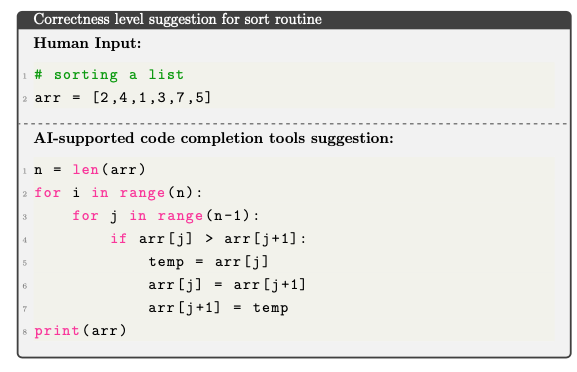
\includegraphics[width=.9\linewidth]{Figures/correctness.png}
    \caption{Code suggestion of \cct{} at correctness level}
    \label{fig:correctness}
\end{figure}

The goal of this software abstraction level in our taxonomy is for a \cct{} to be able to suggest a solution instead of the best one.
The capabilities required by \cct{} to satisfy this level of abstraction are as follows:

\begin{enumerate}
    \item Suggest a solution for a given programming task that may not be the optimal solution for that programming task.
    \item The solution suggested is not required to cover all the edge cases for that programming task.
    \item Satisfy requirements of all the levels below correctness in our taxonomy.
\end{enumerate}

% \begin{tcolorbox}[title=Correctness level suggestion for sort routine,boxsep=.15mm]
%     %https://tex.stackexchange.com/questions/337909/tcolorbox-tcbline-style
% \textbf{Human Input:}
% \begin{lstlisting}[language={Python}]
% # sorting a list
% arr = [2,4,1,3,7,5]
% \end{lstlisting}
% \tcbline
% \textbf{\cct{} suggestion:}
% \begin{lstlisting}[language={Python}]
% n = len(arr)
% for i in range(n):
%     for j in range(n-1):
%         if arr[j] > arr[j+1]:
%             temp = arr[j]
%             arr[j] = arr[j+1]
%             arr[j+1] = temp
% print(arr)
% \end{lstlisting}
% \end{tcolorbox}